\documentclass{article}

% if you need to pass options to natbib, use, e.g.:
%     \PassOptionsToPackage{numbers, compress}{natbib}
% before loading neurips_2020

% ready for submission
% \usepackage{neurips_2020}

% to compile a preprint version, e.g., for submission to arXiv, add add the
% [preprint] option:
\usepackage[preprint]{neurips_2020}

% to compile a camera-ready version, add the [final] option, e.g.:
%     \usepackage[final]{neurips_2020}

% to avoid loading the natbib package, add option nonatbib:
%    \usepackage[nonatbib]{neurips_2020}

\usepackage[utf8]{inputenc} % allow utf-8 input
\usepackage[T1]{fontenc}    % use 8-bit T1 fonts
\usepackage{hyperref}       % hyperlinks
\usepackage{url}            % simple URL typesetting
\usepackage{booktabs}       % professional-quality tables
\usepackage{amsfonts}       % blackboard math symbols
\usepackage{nicefrac}       % compact symbols for 1/2, etc.
\usepackage{microtype}      % microtypography
\usepackage{graphicx}
\usepackage{float}
\restylefloat{table}
\usepackage{array}
\usepackage{booktabs, multirow} % for borders and merged ranges
\usepackage{soul}% for underlines
\usepackage[table]{xcolor} % for cell colors
\usepackage{changepage,threeparttable} % for wide tables
\newcolumntype{L}{>{\centering\arraybackslash}m{3cm}}

\title{Formatting Instructions For NeurIPS 2020}

% The \author macro works with any number of authors. There are two commands
% used to separate the names and addresses of multiple authors: \And and \AND.
%
% Using \And between authors leaves it to LaTeX to determine where to break the
% lines. Using \AND forces a line break at that point. So, if LaTeX puts 3 of 4
% authors names on the first line, and the last on the second line, try using
% \AND instead of \And before the third author name.

\title{Understanding gender violence depiction in online news media}

\author{Caitlin Loftus \\
	\texttt{cloftus@uchicago.edu}  \\
	The University of Chicago
	\AND
	Roberto Barroso-Luque\\
	\texttt{barrosoluquer@uchicago.edu} \\
    The University of Chicago\\
	\AND
	Rukhshan Mian\\
	\texttt{rukhshan@uchicago.edu} \\
	The University of Chicago\\}

\begin{document}
\maketitle

\begin{abstract}{
		Our study blabla
	}
\end{abstract}

\newpage
\section{Introduction and Background}{
	
The declaration on the Elimination of Violence against Women, which was adopted by the United Nations in 1993, defines gender-based violence (GBV) as “any act of gender-based violence that results in, or is likely to result in, physical, sexual or psychological harm or suffering to women, including threats of such acts, coercion or arbitrary deprivation of liberty, whether occurring in public or in private life”. 

“Violence against women and girls is one of the most systematic and widespread human rights violations” according to the United Nations Entity for Gender Equality and the Empowerment of Women (UN Women). According to research by the World Health Organisation, in 2018 1 in 3 women worldwide had been subjected at least once in their lifetime to physical and/or sexual violence from any current or former husband or male intimate partner, or to sexual violence from someone who was not a current or former partner. 

Public  interest  journalism has great potential to help in the fight against  gender-based violence. A recent example of this was the MeToo movement, which largely began as a result of investigations by the New York Times. Despite the potential, the media’s portrayal of gender based violence can also have negative impacts on how society views these types of violence. A literature review found number of key themes in the way news media portray violence against women including “perpetuating myths and misrepresentations”, and “directly and indirectly shifting blame from male perpetrators of violence and assigning responsibility for violence to women”.

The media’s reporting can impact the public’s perception of GBV in a number of different ways. Firstly what is chosen to be reported on influences the types of violence the public are aware of and see as important issues. Secondly, the particular language choices made in the reporting—such as the words chosen to describe GBV, the structure of the writing, and particular linguistic devices—has a big impact on the public’s perception of GBV. For example, previous research has shown that the use of the passive voice in reporting of rape cases removes blame from the attacker (Bohner, 2001). Braber (2014) also demonstrated the use of the the passive voice in newspaper reporting about domestic violence cases, for example “an article in The Guardian describes the killing and the murder of a woman and her daughter, without mentioning the man who killed them.”

Natural language processing (NLP) techniques can be used to further understand the ways in which GBV is reported in the media. NLP techniques allow for easy detection of linguistic patterns over a large corpus, so can be used to test for for the presence of particular linguistic devices, or to detect new patterns. Our research aims to understand the words and language patterns used to describe instances of GBV in newspaper articles, with a focus on semantic meaning of words and on the use of the passive voice. 

For the purpose of our research we look at newspaper articles from Mexico, the UK and Pakistan. In recent years there have been a number of important cases and movements surrounding gender-based violence in these three countries. We include Mexico to understand how GBV movements have been reported in the news and see how political ideologies may impact reporting methods. Instances of GBV are prevalent in the UK as well. Sarah Everard's death in early 2021 set off protests and movements against such instances. The case was reported on in various ways by different news outlets – some resorted to victim-blaming whereas some focused on more in-depth analysis. These patterns have been present in the past as well in terms of what kind of language is being used to depict instances of gender-based violence. Lastly, we take into account Pakistan where GBV is a widely underreported topic. Such instances are highly prevalent and a significant percentage of women experience domestic violence. Causes of underreporting include: A lack of belief in a legal system, lack of accountability in the (policing) authorities to actually report these issues, etc. Victim-blaming is unfortunately the norm in most instances and our goal is to analyze the sort of language news outlets use to describe such cases.

\subsection{Related work}{
The motivation behind looking at passive voice instances in newspaper articles related to GBV stems primarily from pre-existing literature. Research from Germany suggests how passive voice predominates in mass media reports describing male violence against women. Herd (2001) further suggest how content related to GBV tends to put the actor in the background and the acted-upon person in the focus of discourse. This study from Germany found how passive voice positively correlated positively with rape-myth acceptance and perceived responsibility of the victim (Herd 2001). This study was aimed at identifying subtle linguistic indicators of blaming victims of sexual violence, and at relating these to direct judgments of responsibility (Herd 2001). Although the experiment was conducted on non-professional writers, we aim to extend this to look at how relatively professional writers describe cases of gender-based violence. We aim to build on existing literature and delve more into the extent to which passive voice is used in such newspaper articles.

Motivation for this topic also stems from anecdotal evidence. We often see cases of GBV being reported in newspapers. The language used in such articles often places the blame on women. Or rather, the language used intentionally tries to take away from the GBV act. An example of this can be seen here from an
\textcolor{blue}{\href{https://twitter.com/TheSun/status/755867885910851584}{\underline{article}}} published in the Sun, a right-wing newspaper from the UK
The language used is passive and the words being used to describe the instance itself are vague. Attention is being given to what the victim was doing as opposed to focusing on what the perpetrator did. Existing literature combined with such evidence lay the foundation for what we try to explore. Our aim is to look at the extent to which passive voice occurs in GBV-related newspaper articles in Mexico, UK and Pakistan.

First proposed by Harris, in the seminal work Distributional Structure  (1954)  and popularized by Firth (1957)  the Distributional Hypothesis of Language suggests that words that occur in similar contexts have similar meanings and that differences in linguistic form connote differences in meaning. This linguistic theory has given rise to a plethora of subsequent research by which Natural Language Processing methods have been used to understand the semantic meaning of words and concepts in different corpuses. Two recent studies are of particular relevance to our research.

Kozlowski et al. (2019) made use of the exciting method of word embeddings to analyze millions of books published during the span of 100 years and track how the meaning and social context of class shifted amid social transformations.  The authors trained word embedding models on Google Ngrams text from books published over the span of the twentieth century to gain insights into socio-cultural understandings of social class. Surprisingly, this work found that word embeddings which include stereotypes and other harmful biases tend to accurately represent the cultural systems and corresponding text which give rise to such stereotypes. In addition, the authors find that the meaning of terms as represented by word embeddings closely resemble the meaning of these same terms in human responses, based on responses in the cloud-source platform Mechanical Turk. 

Caliskan et al. (2017) use Global Vector representations, or GloVe embeddings to understand historical biases in text across a multitude of dimensions including race and gender. This work finds that there exists a relationship between prejudicial human behavior and the division between ingroup-outgroups which can be understood through the semantic relationships between words in language.

Taken together, these two papers exploit the assumptions of the Distribution Hypothesis of Language to gain insights into complex socio-cultural concepts by creating multidimensional vector representations of human language. We follow a similar methodology by using the Word2Vec algorithm and creating word embeddings of each of our compiled corpus, one language model for each newspaper. In doing so we seek to understand which terms are related to each other by comparing their cosine distance in multidimensional vector space.  This analysis allowed us to understand and compare multiple cultural and social concepts and their relationship to domestic violence in contemporary online media. 
}

}
\newpage

\section{Methodology}{
	
\subsection{Creating our corpus}{
%Please add the following packages if necessary:
%\usepackage{booktabs, multirow} % for borders and merged ranges
%\usepackage{soul}% for underlines
%\usepackage[table]{xcolor} % for cell colors
%\usepackage{changepage,threeparttable} % for wide tables
%If the table is too wide, replace \begin{table}[!htp]...\end{table} with
%\begin{adjustwidth}{-2.5 cm}{-2.5 cm}\centering\begin{threeparttable}[!htb]...\end{threeparttable}\end{adjustwidth}

For our analysis we needed a corpus of newspaper articles related to GBV. No such corpus was already available, so we compiled our own using web scraping techniques. We identified a number of keyword search terms related to GBV which we used to scrape article data from newspaper websites. 

\subsubsection{Selecting relevant keyword search terms}{
To generate our list of keyword search terms, we initially based our list on some previous work done by Rukhshan, and then refined and added to the list based on our understanding from the literature. On coming up with the list of search terms we had two key things in mind: firstly GBV is quite broadly defined, so we wanted a list of search terms that reflected the range of different forms of gender based violence; secondly we identified search terms specific to GBV that we could be reasonably confident would return only relevant articles. 

This process gave us a list of 10 relevant keywords in English, and Roberto then compiled a list of Spanish search terms that closely matched the English list. The search terms used are as follows:

English: "rape", "gang-rape", "gender-based violence", "child+abuse", "forced+marriage", "forced+abortion", "sexual+assault", "domestic+violence", "sexual+abuse", "woman+murder", "honor+killing"

Spanish: "violencia+genero", "asesinato+mujer", "matrimonio+forzado", "aborto+forzado", "agresion+sexual", "violencia+domtica", "abuso+sexual", "Feminicidio"
                }
\subsubsection{Selecting the newspapers}{ 
In selecting the newspapers to scrape article data from, we wanted to get a roughly even number of articles from each of the three countries, and we also wanted to select newspapers from across the ideological spectrum in each country. We identified three popular newspapers from each of the countries to gather data on. The newspapers chosen, their political ideological tilt, and the number of articles scraped from them can be viewed in Table 1 below.

For Pakistan we chose to only select articles that were written in English. This is because the highly cursive nature of Urdu would make it difficult to process in NLP models. The major news sources in Pakistan also primarily publish articles written in English, and the Urdu versions are often uploaded as images so it would require more complicated technologies to extract the information.

Furthermore, our selection of Mexican newspapers is based on the work of Rodelo and Muniz (2016) in which they explore ideological and political tilt among the fifteen most read newspapers in Mexico. We selected El Heraldo, El Universal and La Jornada as paragon examples of conservative, moderate and left ideologies in mexican journalism.}

\subsubsection{Web scraping}{
To gather the data we primarily used Selenium and Beautiful Soup in Python to scrape the article data for each keyword for each identified newspaper. One of the news sources we had chosen (the Guardian from the UK) has their own api, which we used to collect that data. To scrape the data we passed each of our search terms into the search functionalities on the newspaper websites, and scraped the article data for the returned search results. 

We scraped articles that were published from the beginning of 2020 until the present day. This was because we were interested in recent events in each country. Our article collection gave us a corpus of around 17,700 articles on topics related to GBV. You can see the breakdown of the number of articles by newspaper in Table 1.}

\begin{table}[!htp]\centering
	\caption{Article and Newspaper Counts}\label{tab: }
	\scriptsize
	\begin{tabular}{lrrrr}\toprule
		&\textbf{Newspaper} &\textbf{Political ideology} &\textbf{Number of articles} \\\midrule
		\multirow{3}{*}{Mexico} &El Heraldo &Right &2820 \\
		&El Universal &Centre &3513 \\
		&La Jornada &Left &2099 \\
		& & & \\
		\multirow{3}{*}{Pakistan} &Nation &Centre-Right &968 \\
		&Dawn &Centre-Left &330 \\
		&The News &Centre-Left &930 \\
		& & & \\
		\multirow{3}{*}{UK} &The Times &Centre-right &1206 \\
		&The Sun &Right &1269 \\
		&The Guardian &Left &4568 \\
		& & & \\
		Total & & &17778 \\
		\bottomrule
	\end{tabular}
\end{table}

\subsubsection{Data cleaning}{
After compiling our copus, the data needed cleaning and normalising before we could use it for our analyses. We removed any duplicate articles, and then pre-processed the data using methods such as stop-word removal, tokenizing and normalising.}

}

\subsection{GBV NN Classification}{
On beginning our analyses we noticed there appeared to be some noise in our data, as some article headlines did seem to be related to GBV. To investigate this we first took a random sample of 100 headlines each from four of our newspaper datasets and manually labelled the headlines as related to GBV, not related to GBV, or unclear. You can see the breakdown of this initial labelling in Table 2.

\begin{table}[!htp]\centering
	\caption{Noise in newspaper headlines initial counts (out of 100)}\label{tab: }
	\scriptsize
	\begin{tabular}{lrrrr}\toprule
		&Yes &No &Unsure \\\midrule
		Pakistan combined &58 &28 &14 \\
		UK - the Sun &64 &27 &9 \\
		UK - the Times &50 &40 &10 \\
		UK - the Guardian &30 &58 &12 \\
		\bottomrule
	\end{tabular}
\end{table}

The noise in our data is a result of methods we used to collect our data. By scraping data using a keyword search we are reliant on each website’s search functionality. This can cause noise in the data for two different reasons. Firstly each website has their own way they prioritise results from search requests. This means that if we have a composite search term such as “domestic+violence”, some websites will prioritise articles with the full search term in the results, whereas others also return results where the individual words (“domestic” and “violence”) are present separately. Secondly, a keyword search returns articles where that keyword term is present anywhere in the article, even if it is not the main focus of the article. This means that when looking at the headline of an article it may not appear to be about GBV even though a GBV keyword term is present somewhere in the article. 

From the results of the initial headline labelling it was clear that noise in our data was a concern, so we decided to build a binary classification model to attempt to filter out the noise from the corpus. To do this we created a labelled dataset of a random subset of the data and built a recurrent neural network model in PyTorch

\subsubsection{Labelling the data}{
We chose to take a random sample of 300 articles from each of our newspaper datasets to label and use to train our classification model. This gave us around 900 articles from each country to be split into train, test and validation sets. This number was chosen so as to be manageable to label as we were manually labelling the data while giving us enough data to meaningfully train our model. 

We labelled the data based mainly on the article headline, and on the article text if the context was not clear from the headline. We used binary labels, where an article was labeled with a 1 we determined it was about GBV, and 0 otherwise. You can view the breakdown of the percentage of articles labelled as 1 (about GBV) by newspaper in Table 3 below.

\begin{table}[!htp]\centering
	\caption{Percentage of GBV articles in corpus by newspaper (out of 300 articles for each newspaper)}\label{tab: }
	\scriptsize
	\begin{tabular}{lrrr}\toprule
		&\textbf{Newspaper} &\textbf{GBV articles (\%)} \\\midrule
		\multirow{3}{*}{Mexico} &El Heraldo &70 \\
		&El Universal &77 \\
		&La Jornada &69 \\
		& & & \\
		\multirow{3}{*}{Pakistan} &Nation &63 \\
		&Dawn &77 \\
		&The News &74 \\
		& & & \\
		\multirow{3}{*}{UK} &The Times &48 \\
		&The Sun &65 \\
		&The Guardian &37 \\
		\bottomrule
	\end{tabular}
\end{table}

}

\subsubsection{Binary classification model}{

For our classification model we chose to create a Long-Short Term Memory (LSTM) model (Hochreiter and Schmidhuber, 1997). An LSTM model is a recurrent neural network with a gating mechanism. This means that unlike feedforward neural networks an LSTM model has backwards connections, which allows the model to learn the whole context of a sentence, and how the words relate to each other. The gating mechanism allows for some information held in memory in the model to be forgotten, so only the relevant information is retained. 

We created the LSTM binary classification model in PyTorch, using the article headlines as the text input, and the binary labels we had assigned as the target output. We normalized the headline text and tokenized it using the SpaCy tokenizer. An example of the data after tokenizing is as follows, with ‘text’ containing the tokenized headline, and the label being the label we had assigned:

\begin{verbatim}
{'text': ['sarah', 'everard', 'met', 'officer', 'appears', 'in', 'court',
'charged', 'with', 'kidnap', 'and', 'murder'], 'label': 1}    
\end{verbatim}

We created a separate model for each country. For Mexico this makes sense as the articles are in Spanish whereas the UK and Pakistan articles are in English. While building the models we also discovered that article headlines are written quite differently in newspapers from Pakistan as compared to those from the UK and the models learnt better when we created separate models for articles from Pakistan and from the UK.  

The LSTM model was defined with the following parameters:
\begin{itemize}
  \item Embedding layer: length of the input vocab x the embedding dim, with a padding index of 1
  \item LSTM layer: embedding dim x hidden dim, with a dropout rate of 0.2
  \item Linear layer 1: 2x hidden dim x hidden dim
  \item Linear layer 2: hidden dim x 1, with a dropout rate of 0.2 
\end{itemize}

For example, for the Pakistan model the parameters were as follows:
\begin{verbatim}
LSTM_net(
  (embedding): Embedding(1371, 200, padding_idx=1)
  (lstm): LSTM(200, 256, num_layers=2, batch_first=True, dropout=0.2,
               bidirectional=True)
  (fc1): Linear(in_features=512, out_features=256, bias=True)
  (fc2): Linear(in_features=256, out_features=1, bias=True)
  (dropout): Dropout(p=0.2, inplace=False)
)\end{verbatim}

For the two English language models (Pakistan and the UK), we trained two models: one where we initialised the embedding layer with GloVe embeddings, and another where we initialised the embedding layer randomly. For the Mexico model we were not able to find appropriate pre-trained embeddings, so only one model was trained on the Mexican articles. 
}

}

\subsection{Word2Vec and Sentiment Analysis}{

We used the Word2Vec algorithm introduced by Mikolov et al (2013) to create word embedding representations of each of the newspaper corpus we compiled. The raw text from each document (e.g., an article for each newspaper in our dataset) was tokenized
and normalized using word-tokenize and sentence-tokenize methods in Python. Sentence tokenized documents were retained in order to create a continuous bag of words (CBOW) representation of each newspaper corpus using Gensim’s implementation of the Word2Vec algorithm.

Once created, word embedding models for each of the newspapers were visualized using Principal component analysis and TSNE. PCA was used to create linear mappings of the multi-dimensional WE models by reducing each WE representation into the ten principal component vectors. The first two principal components were then plotted as well as a scree plot to understand the variance explained by each PC vector. Due to the linear limitations of PCA, we decided to employ TSNE to create a non linear low-dimensional representation of our high-dimensional WE spaces (Figures 1-6). Keywords were then selected and highlighted in both PCA and TSNE plots to understand their relationship to other keywords and the corpus in general. By observing the relative distance between keywords in these lower dimensional spaces we then made inferences of semantic meaning for each keyword and comparisons of their use across the political spectrum.

Furthermore, we made use of pre-trained neural network sentiment models in order to understand the relative polarity of keywords in each corpus. In order to get the average polarity of words in a specific corpus, we iterated over each keyword and over each WE model finding the closest words,  based on cosine similarity, for each keyword i in each WE model j. We then used VaderSentiment’s pre-trained model to evaluate polarity for the ten “closest” words and assigned the average polarity to their respective keywords. Moreover, we used the same methodology with pre-trained Glove Embeddings (English) and the Spanish Billion Word Embeddings (Spanish) as points of comparison for the relative polarity of our keywords in their respective languages. 

Finally, semantic algebra using the vector representation of specific words was used to create an analogy solver as proposed by Mikolov et al (2013). Using this methodology we investigated the analogy of woman: victim as man: ?? as described in (equation 1). 

\begin{equation} \label{eu_eqn}
	analogy(m:w \rightarrow k:?) = argmax_{v,w,k}(cos(v,k)-cos(v,m)+cos(v,w)))
\end{equation}

}


\subsection{Passive Voice}{
Before delving into how we go about identifying passive voice patterns in our corpus, we define what passive voice and, for comparison, active voice are.

\begin{itemize}
    \item \textbf{Passive Voice}: In this case, the subject is a recipient of a verb’s action (target + verb + actor) Examples of passive voice would be:
    \begin{itemize}
        \item Spanish: El libro fue escrito por Emilio.
        \item English: The book was written by Emilio
    \end{itemize}

    \item \textbf{Active Voice}: Case where sentence has a subject that acts upon its verb (actor + verb + target) Examples of active voice would be:
    \begin{itemize}
        \item Spanish: Emilio escribe un libro.
        \item English: Emilio is writing a book.
    \end{itemize}
\end{itemize}

In the aforementioned examples, we observe how active sentences are easier to read and understand. Passive sentences have an associated ambiguity associated with them and are structured in a complex manner. Thus, in order to identify a sentence with passive voice, we would need to analyze the grammatical structure of a sentence based on the dependencies between the words. This is possible through dependency trees that allow us to recognize a sentence and then assign a syntactic structure to it.

In order to understand dependencies, we look at an example sentence:

\begin{center}\emph{“Dependencies for Bills on ports and immigration were submitted by Senator Brownback, Republican of Kansas”}
\end{center}

Firstly, we observe that this sentence is in the passive voice. It follows 
has a fairly complex structure. The dependency tree for this sentence is given in the following image:


\begin{figure}[H]
	\center{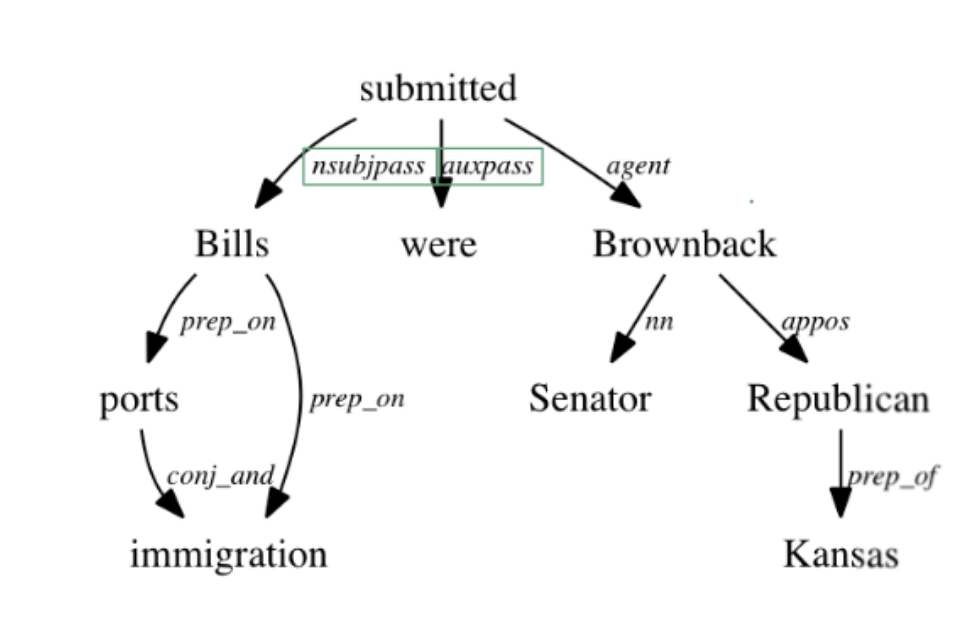
\includegraphics[width=\textwidth]
		{figures/deptree.png}}
	\caption{\label{fig:my-label1} Dependency tree for an example sentence. Source(Stanza Documentation)}
\end{figure}

The labels next to the arrows in the tree are the dependencies. We observe multiple in this sentence however our focus is on the dependencies in green boxes: \emph{nsubjpass} (passive nominal subject) is a noun phrase which is the syntactic subject of a passive clause. \emph{auxpass} (auxiliary passive clause) is  non-main verb of the clause which contains the passive information

Moving forward with these definitions in mind, we observe how the word submitted, in this context, occurs as an \emph{nsubjpass} whereas the word were occurs as an \emph{auxpass}. The occurrence of these two together is what we define as a passive instance.

To solidify how we define a passive instance, we took a list of passive sentences in Spanish and English and created dependency trees using Stanza – which contains pre-trained neural network models supporting both languages. We used these trees to perform a manual check of patterns that only appeared in passive sentences (in both Spanish and English). Using this method, we arrived at the following patterns for Spanish: ['det', 'nsubj', 'aux', 'root'], ['det', 'nsubj', 'advmod', 'aux', 'aux', 'root'], ['det', 'nsubj', 'amod', 'aux', 'root'], ['det', 'nsubj', 'aux', 'root', 'case', 'det'], 'explpass'. For English, we arrive at the following pattern: [nsubjpass, auxpass].

Having identified these patterns, we created pipelines in Stanza for Spanish, combined the article headline and text and looked for the number of times these patterns occur in our data. For the purpose of this analysis, we kept 300 articles from each newspaper. Once we arrived at the count of passive instances, we divided these up by the number of sentences in that article – this allowed us to have a normalized estimate that we could easily interpret.

One limitation to our approach is that passive voice in a sentence may exhibit patterns that we have not accounted for. Furthermore, to make our methodology more rigorous, an LSTM could be implemented. However, for this purpose, a larger pre-labelled dataset with passive sentences (related to gender-based violence newspaper articles) would be required. These were not available online and these would thus need to be manually labelled. Although these limitations are necessary for us to consider, our goal is to lay the foundation for future research in passive voice depiction in GBV-related newspaper articles. Results are discussed in the next section.

}
}


\section{Results}{	
\subsection{Semantic Meaning in Word Embedding Models}{
	
As described in our methodology section, we visualized the relationship between words in our corpus using PCA and TSNE. Specifically, we focused on the relationship of a set of keywords (equation 2) and their direct translation to spanish. 

\begin{equation} \label{eu_eqn}
	w \in \sqsubset  {man, woman, abuse, place, victim, blame, responsibility} \sqsupset
\end{equation}

Figure 1 and Figure 2 show examples of PCA, TSNE and scree plots for a word embedding models fit to The Guardian (UK) and The Sun (UK) newspapers. We find that the relative distance between specific keywords such as woman, abuse and man in The Guardian WE model (Figure 1) when compared to the relative distance to the same three words in The Sun WE model (Figure 2) and The Times WE model (Supplementary Figure 5) show differential semantic use of these three words by each newspaper. The Guardian, which is left of center in the political spectrum, associates the word man as a middle word between abuse and woman as seen in the central position found in its WE model. In contrast, The Sun, the most conservative  UK newspaper in our dataset, creates a much closer association between woman and abuse, placing man farther away as seen in the PCA plot for this newspaper. The Times, a moderate UK newspaper, follows a similar pattern to the Guardian. The finding in the UK using relative position of man, abuse and woman is not replicated neither in Pakistan nor in Mexico’s WE models. The appendix shows supplementary figures 4, 5 and 6 with 2-dimensional visualizations for all newspapers grouped by political tilt for all three countries. For both Pakistani and Mexican newspapers it is difficult to draw conclusions from the PCA and TSNE plots of their respective embeddings. Yet by using sentiment analysis and semantic algebra interesting patterns start to arise. 

\begin{figure}[H]
	\center{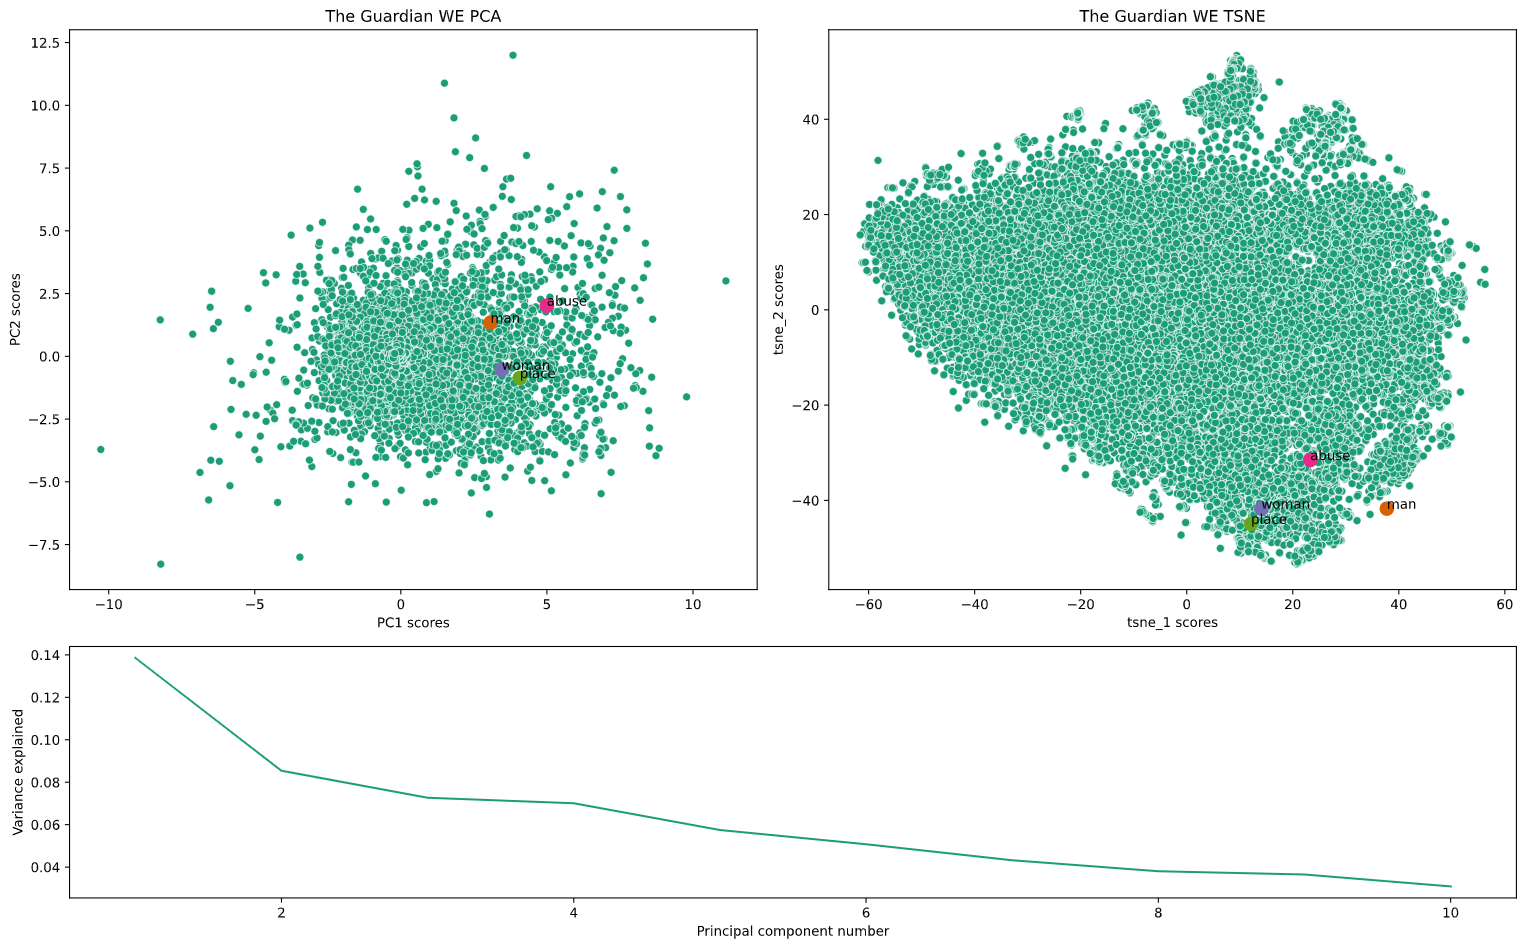
\includegraphics[width=\textwidth]
		{figures/theguardian.png}}
	\caption{\label{fig:my-label1} Visualization of embedding space (The Guardian UK)}
\end{figure}

\begin{figure}[H]
	\center{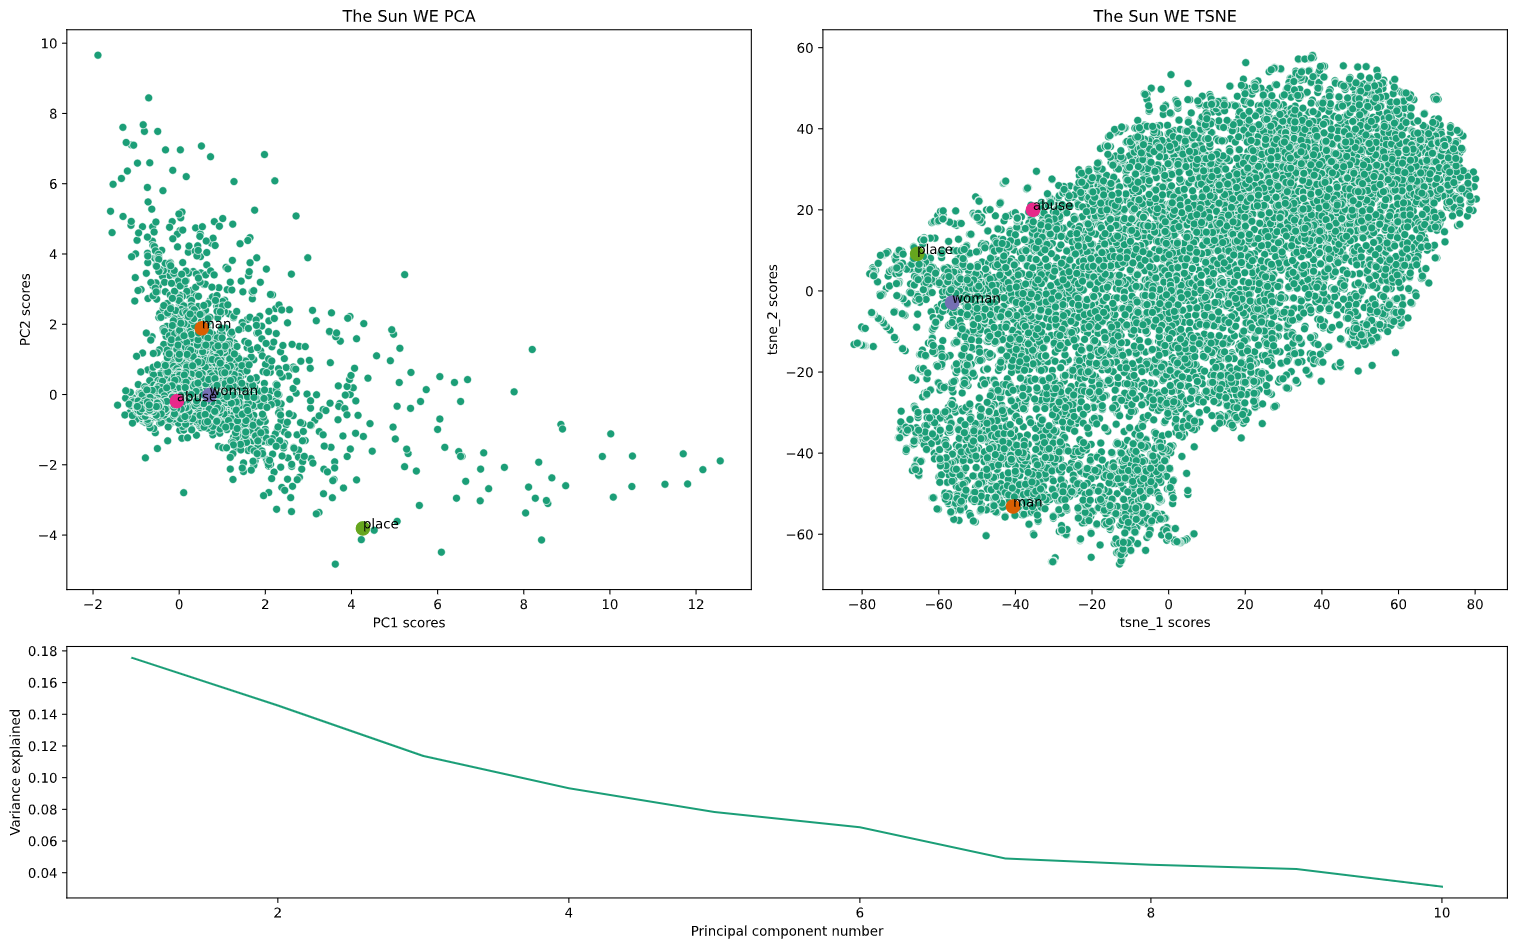
\includegraphics[width=\textwidth]
		{figures/thesun.png}}
	\caption{\label{fig:my-label1} Visualization of embedding space (The Sun)}
\end{figure}


When using semantic algebra to create a word analogy solver (equation 1) we find a clear relationship between ideological tilt and semantic meaning for man and woman in media depictions of GBV. In Table 4 we see the results of the analogy operation for the vector representations of woman, victim and man as described in (equation 3).

\begin{equation} \label{eu_eqn}
	w_{woman} + w_{victim} - w_{man} = ??
\end{equation}

When focusing on the results for newspapers in Mexico, we find that the words that best solve the analogy for right wing newspaper el Heraldo are “expresion”, “condicion”, “completa” (complete). The solution to the same analogy for the moderate El Universal are “libre” (free), “crueldad” (cruelty), “erradicar” (eradicate), etc. While the solutions in La Jornada’s WE representation are “subordinacion” (subordination), “violenta” (violence), “castigar”(punishment), etc. In a similar fashion, when looking at the same analogy for UK newspapers, the words that best solve the analogy in The Guardian embeddings are words such as “perpetrator”, “abuser”, etc. while the words that best solve the analogy in The Sun embeddings are “domestic”, “harassment” etc. This pattern, which we consider one of the critical findings in our work,  suggests that when solving for analogies,  moving from right to left in the political spectrum, there is an increased association of a blame/attacker dimension attributed to man in the lexical space for both Mexican and UK newspapers. This finding is not replicated in the WE representation of Pakistani newspapers. 


%Please add the following packages if necessary:
%If the table is too wide, replace \begin{table}[!htp]...\end{table} with
\begin{table}[!htp]\centering
	\caption{Semantic Algebra: $w_{woman}+ w_{victim} - w_{man} = ??$}\label{tab: }
	\scriptsize
	\begin{tabular}{lrrrr}\toprule
		&\textbf{Newspaper} &\textbf{Political ideology} &\textbf{Result} \\\midrule
		\multirow{3}{*}{Mexico} &El Heraldo &Right &('expresión', 0.91), ('condición', 0.90), ('completa', 0.89), ('ideología', 0.88), ('conlleva', 0.88) \\
		&El Universal &Centre &('libre', 0.92), ('política', 0.92), ('manpowergroup', 0.92), ('crueldad', 0.92), ('erradicar', 0.92) \\
		&La Jornada &Left &('definición', 0.82), ('subordinación', 0.82), ('violenta', 0.81), ('mujerla', 0.81), ('castiga', 0.80) \\
		& & &\textbf{} \\
		\multirow{3}{*}{Pakistan} &Nation &Centre-Right & \\
		&Dawn &Centre-Left &('report', 0.99), ('police', 0.99), ('law', 0.99), ('state', 0.99), ('society', 0.9998923540115356) \\
		&The News &Centre-Left &[('domestic', 0.99), ('harassment', 0.99), ('country', 0.99), ('increase', 0.99), ('rise', 0.99) \\
		&\textbf{} &\textbf{} &\textbf{} \\
		\multirow{3}{*}{UK} &The Sun &Right &('survivor', 0.75), ('domestic', 0.75), ('harassment', 0.73), ('demand', 0.71), ('mutilation', 0.71) \\
		&The Times &Centre-right &('charge', 0.99), ('offence', 0.99), ('allege', 0.99), ('violence', 0.99), ('report', 0.99) \\
		&The Guardian &Left &('survivor', 0.71), ('perpetrator', 0.53), ('domestic', 0.49), ('abuser', 0.48), , ('stalker', 0.44) \\
		\bottomrule
	\end{tabular}
\end{table}

Finally, we go on to use pre-trained sentiment scoring models to find the average polarity of words in our keyword list for each newspaper in our dataset. In addition, we plot the results for the same analysis using the ubiquitous Glove embeddings and Spanish Billion Word (SBW) embeddings. Figure 3 highlights the results of this analysis. One interesting finding is the polarity relationship between newspaper embeddings and the topic agnostic Glove and SBW embeddings. In both Mexico and Pakistan, we find high variance across all newspapers and no obvious correlation between the relative polarity of any one newspaper with Glove or SBW. Nonetheless, in the UK we find that, on average, the polarity of keywords in The Guardian’s WE model tends to mirror, for most words, the polarity found in Glove embeddings. These results might be due to noise artifacts in our data generating process or could provide insights into the general semantic style employed by each newspaper when reporting on GBV. Because of the limitations in inferring semantic meaning in the respective depiction of GBV in our dataset we sought to further understand our corpus through passive/active voice detection.

\begin{figure}[H]
	\center{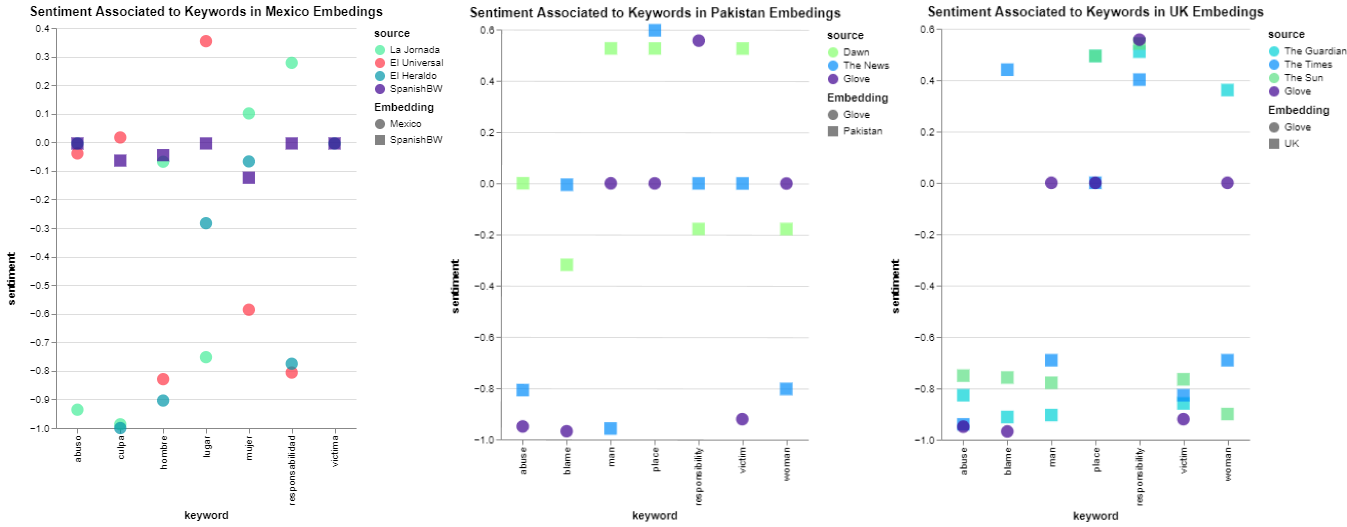
\includegraphics[width=\textwidth]
		{figures/sentimentfig.png}}
	\caption{\label{fig:my-label1} Sentiment towards keywords}
\end{figure}

}


\subsection{Active Passive Voice}{


Using a normalized estimate, we find that approximately 25\% of the content in one article contains some form of passive instance associated with it in Mexican newspapers. In the case of the UK, we find that approximately 31\% of the content in one article contains passive instances. The number for Pakistan is also ~31\%. This is in line with what pre-existing literature suggests. Gerd Bohner in his research based in Germany suggests that passive voice forms about 15\% of the content in an article compared to active voice. We do see that in our case, the estimates are higher. This could primarily be due to the nature of our data collection and our focus on Mexico, UK and Pakistan.

The breakdown by newspaper and political ideology is as follows:

\begin{table}[!htp]\centering
	\caption{Percentage by Newspaper and Political Ideology}\label{tab: }
	\scriptsize
	\begin{tabular}{lrrrr}\toprule
		&\textbf{Newspaper} &\textbf{Political ideology} &\textbf{Result} \\\midrule
		\multirow{3}{*}{Mexico} &El Heraldo &Right &25.7\% \\
		&El Universal &Centre &20.5\% \\
		&La Jornada &Left &25.6\%\\
		& & &\textbf{} \\
		\multirow{3}{*}{Pakistan} &Nation &Centre-Right &29.3\% \\
		&Dawn &Centre-Left &31.5\% \\
		&The News &Centre-Left &32.5\% \\
		&\textbf{} &\textbf{} &\textbf{} \\
		\multirow{3}{*}{UK} &The Sun &Right &25.8\% \\
		&The Times &Centre-right &31.3\%\\
		&The Guardian &Left &35.7\%\\
		\bottomrule
	\end{tabular}
\end{table}

 
 We do not observe any trends in terms of political affiliation and usage of passive voice. Overall, we observe that content from Mexico related to GBV uses less passive voice. This could potentially be as a result of the patterns we use when looking for passive voice.

}


\subsection{LSTM Binary Classifier}{

For the Pakistan and UK models we found they learnt much faster when the embedding layer was initialised with GloVe embeddings, so we chose to use the GloVe embeddings in our final models. You can see the validation accuracy across EPOCH for the two Pakistan models in Figure 5 below. 

The learning rate was similar for the UK, but slightly worse than for Pakistan. The validation accuracy plots for the UK models can be viewed in the Appendix in Figure 9, and the validation accuracy plot for the Mexico model can be viewed in Figure 10 also in the Appendix. 

Our models were learnt to classify article headlines as related to GBV or not with a reasonably high degree of accuracy. Table 6 shows the test set accuracy and F1 scores for the best model for each country. The Mexico model did not learn to classify the headlines as well as the models for the other two countries. This is likely in part due to not initialising the embedding layer with pre-trained embeddings. There may also be other aspects of the model that do not work as well with the Spanish language.


\begin{figure}[H]
	\center{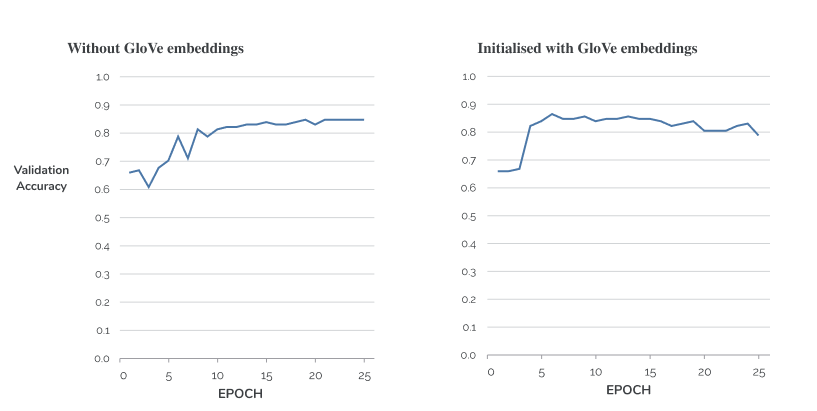
\includegraphics[width=\textwidth]
		{figures/pakistan_validation_accuracies.png}}
	\caption{\label{fig:my-label1} Pakistan LSTM models validation accuracy by EPOCH}
\end{figure}

}
\begin{table}[!htp]\centering
	\caption{Evaluation Metrics LSTM GBV Classifier}\label{tab: }
	\scriptsize
	\begin{tabular}{lrrr}\toprule
		&Test set accuracy &Test set F1 score \\\midrule
		UK best model &0.78 &0.83 \\
		Pakistan best model &0.83 &0.88 \\
		Mexico best model &0.74 &0.71 \\
		\bottomrule
	\end{tabular}
\end{table}
	
}
\newpage
\section{Conclusion, further research and limitations}{
BLABLABLA
}

\newpage
\raggedbottom
\section{Description of effort}{

NEED TO WRITE THIS SECTION!!

Description of your effort, including the relative effort on different activities. 
What did you have to learn for the project? 
What skills did you already possess? E.g., did you need to learn how to use particular libraries? Did you spend more time reading research papers, or fine tuning your parameters? 

\paragraph{What part of the work was done by which team member?}{
\begin{itemize}
  \item Web-scraping and gathering data – Everyone
  \item Word2Vec/Embeddings – Roberto
  \item Classification – Caitlin
  \item Passive Voice – Rukhshan
  \item Presentation + Report – Collectively
\end{itemize}

}
}

\newpage
\section{Appendix}{

\begin{figure}[H]
	\center{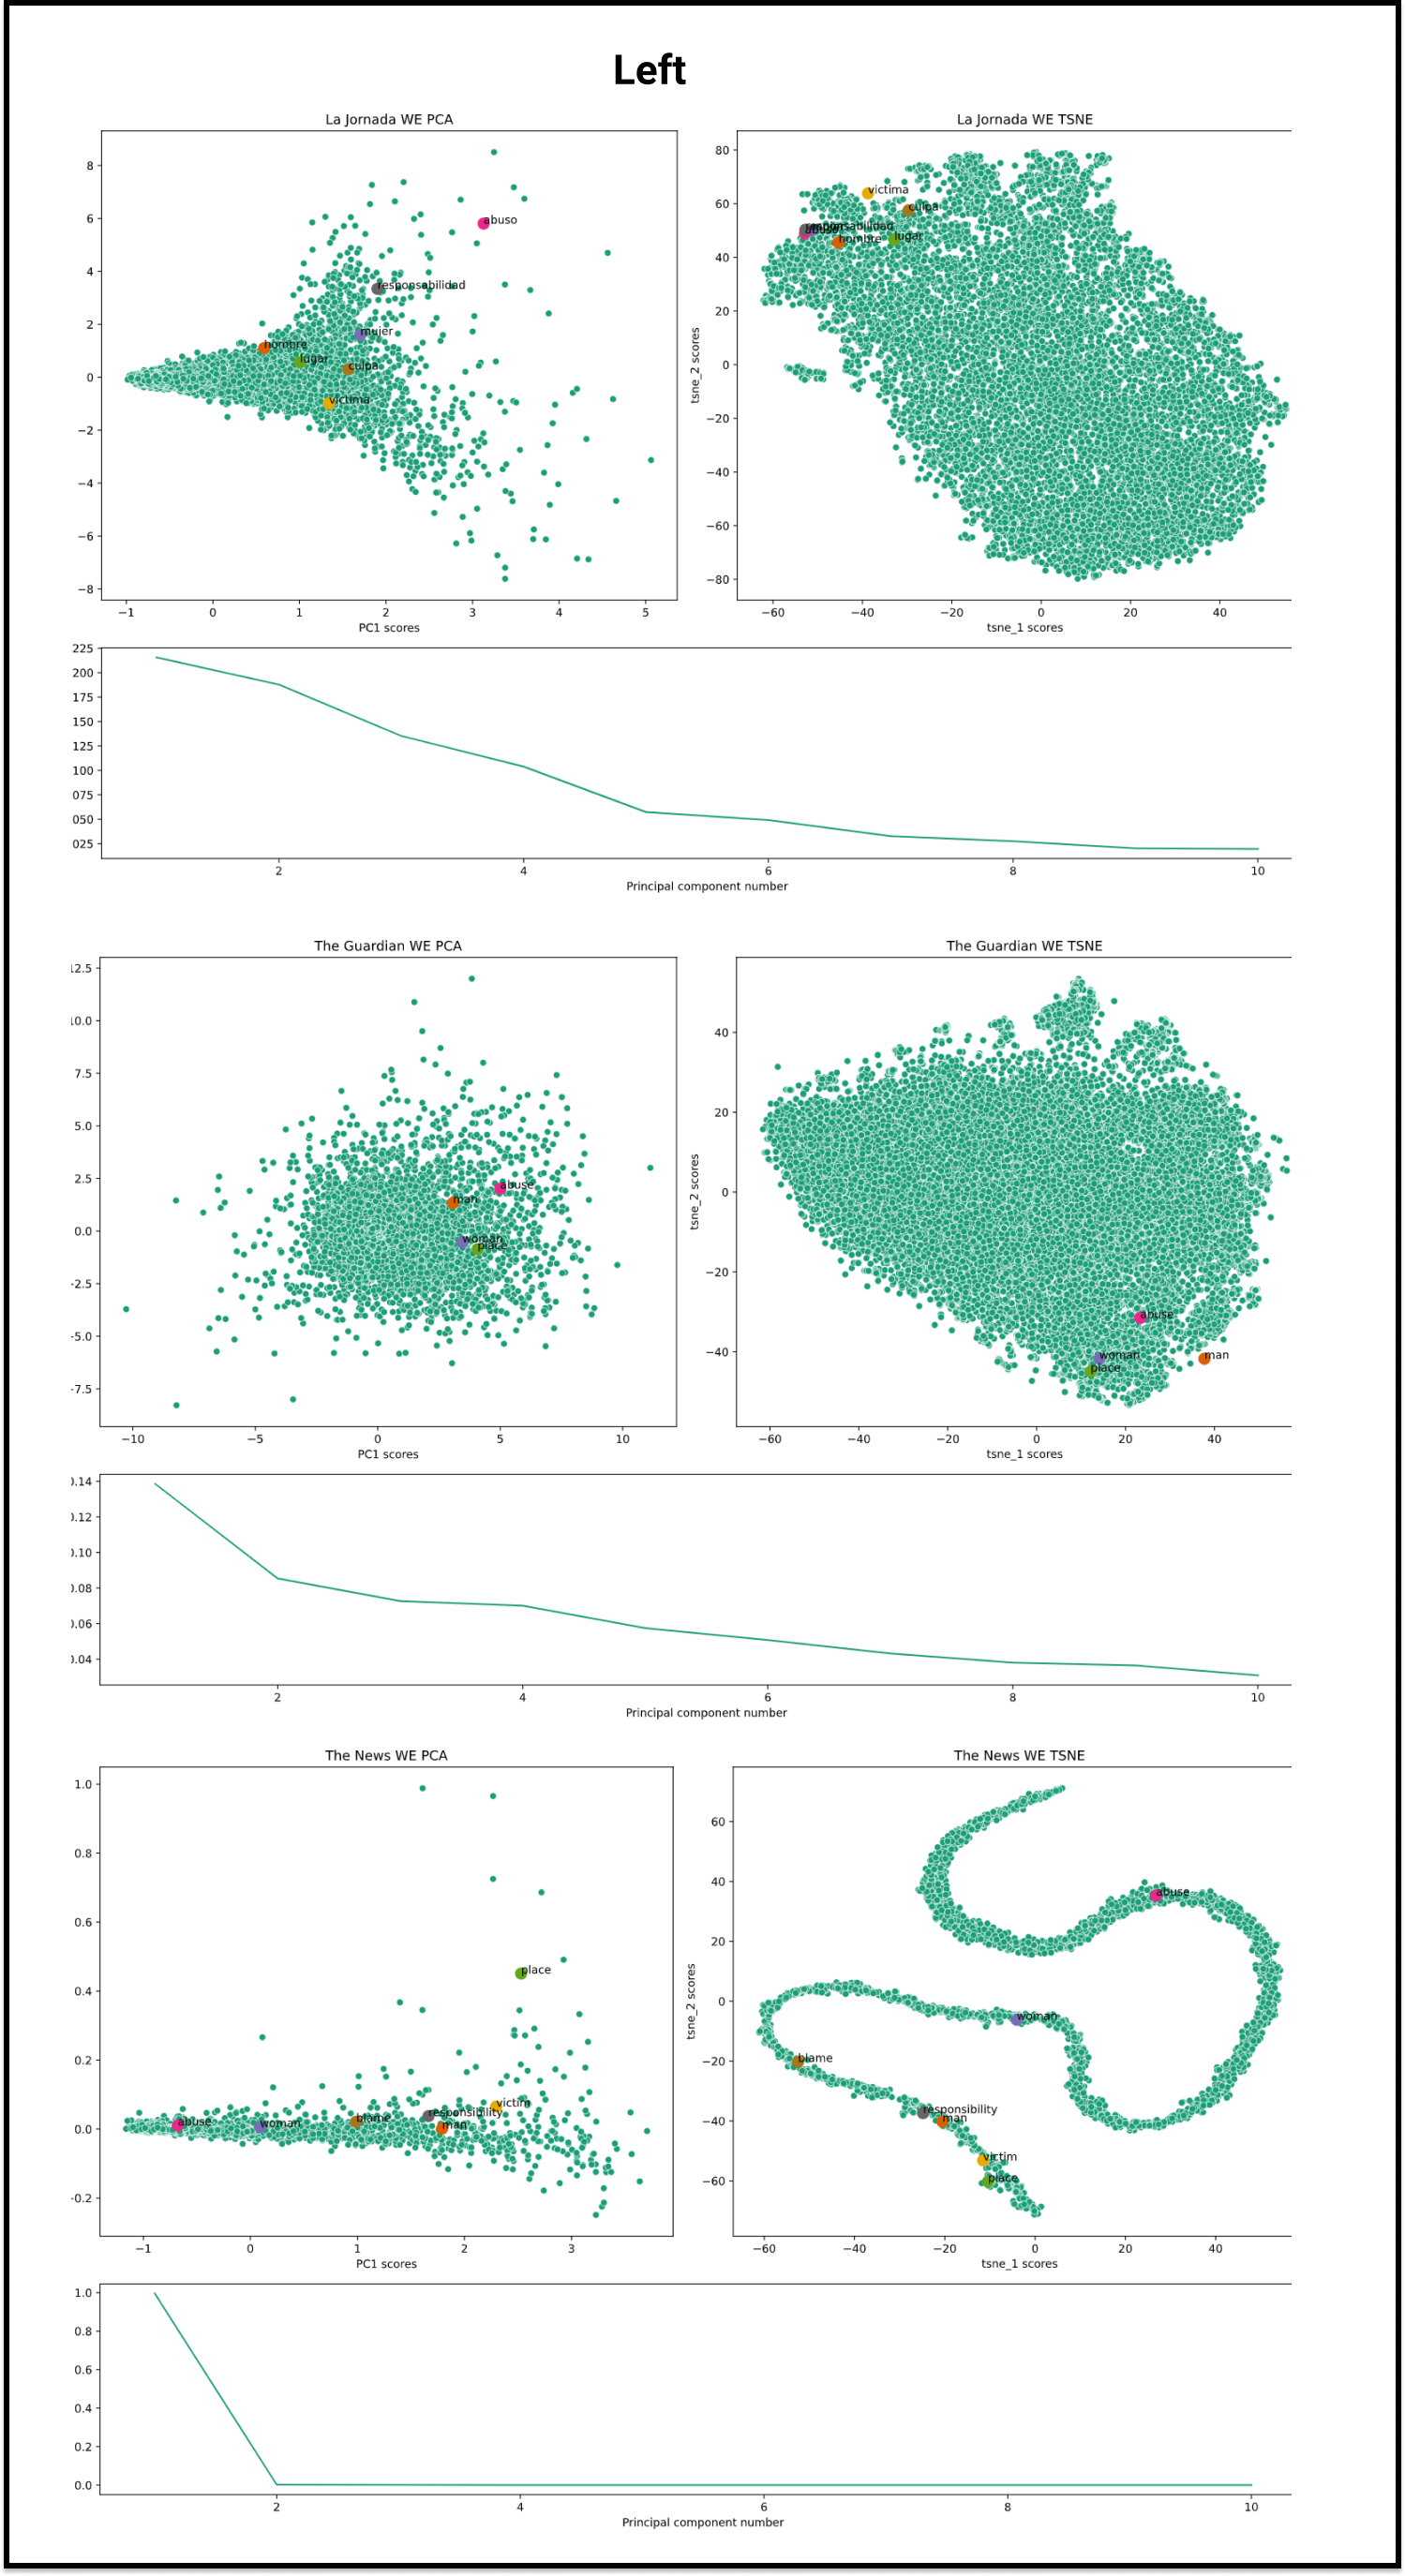
\includegraphics[width=\textwidth,height=\textheight,keepaspectratio]
		{figures/leftwe.png}}
	\caption{\label{fig:my-label1} GBV depiction in left leaning media}
\end{figure}


\begin{figure}[H]
	\center{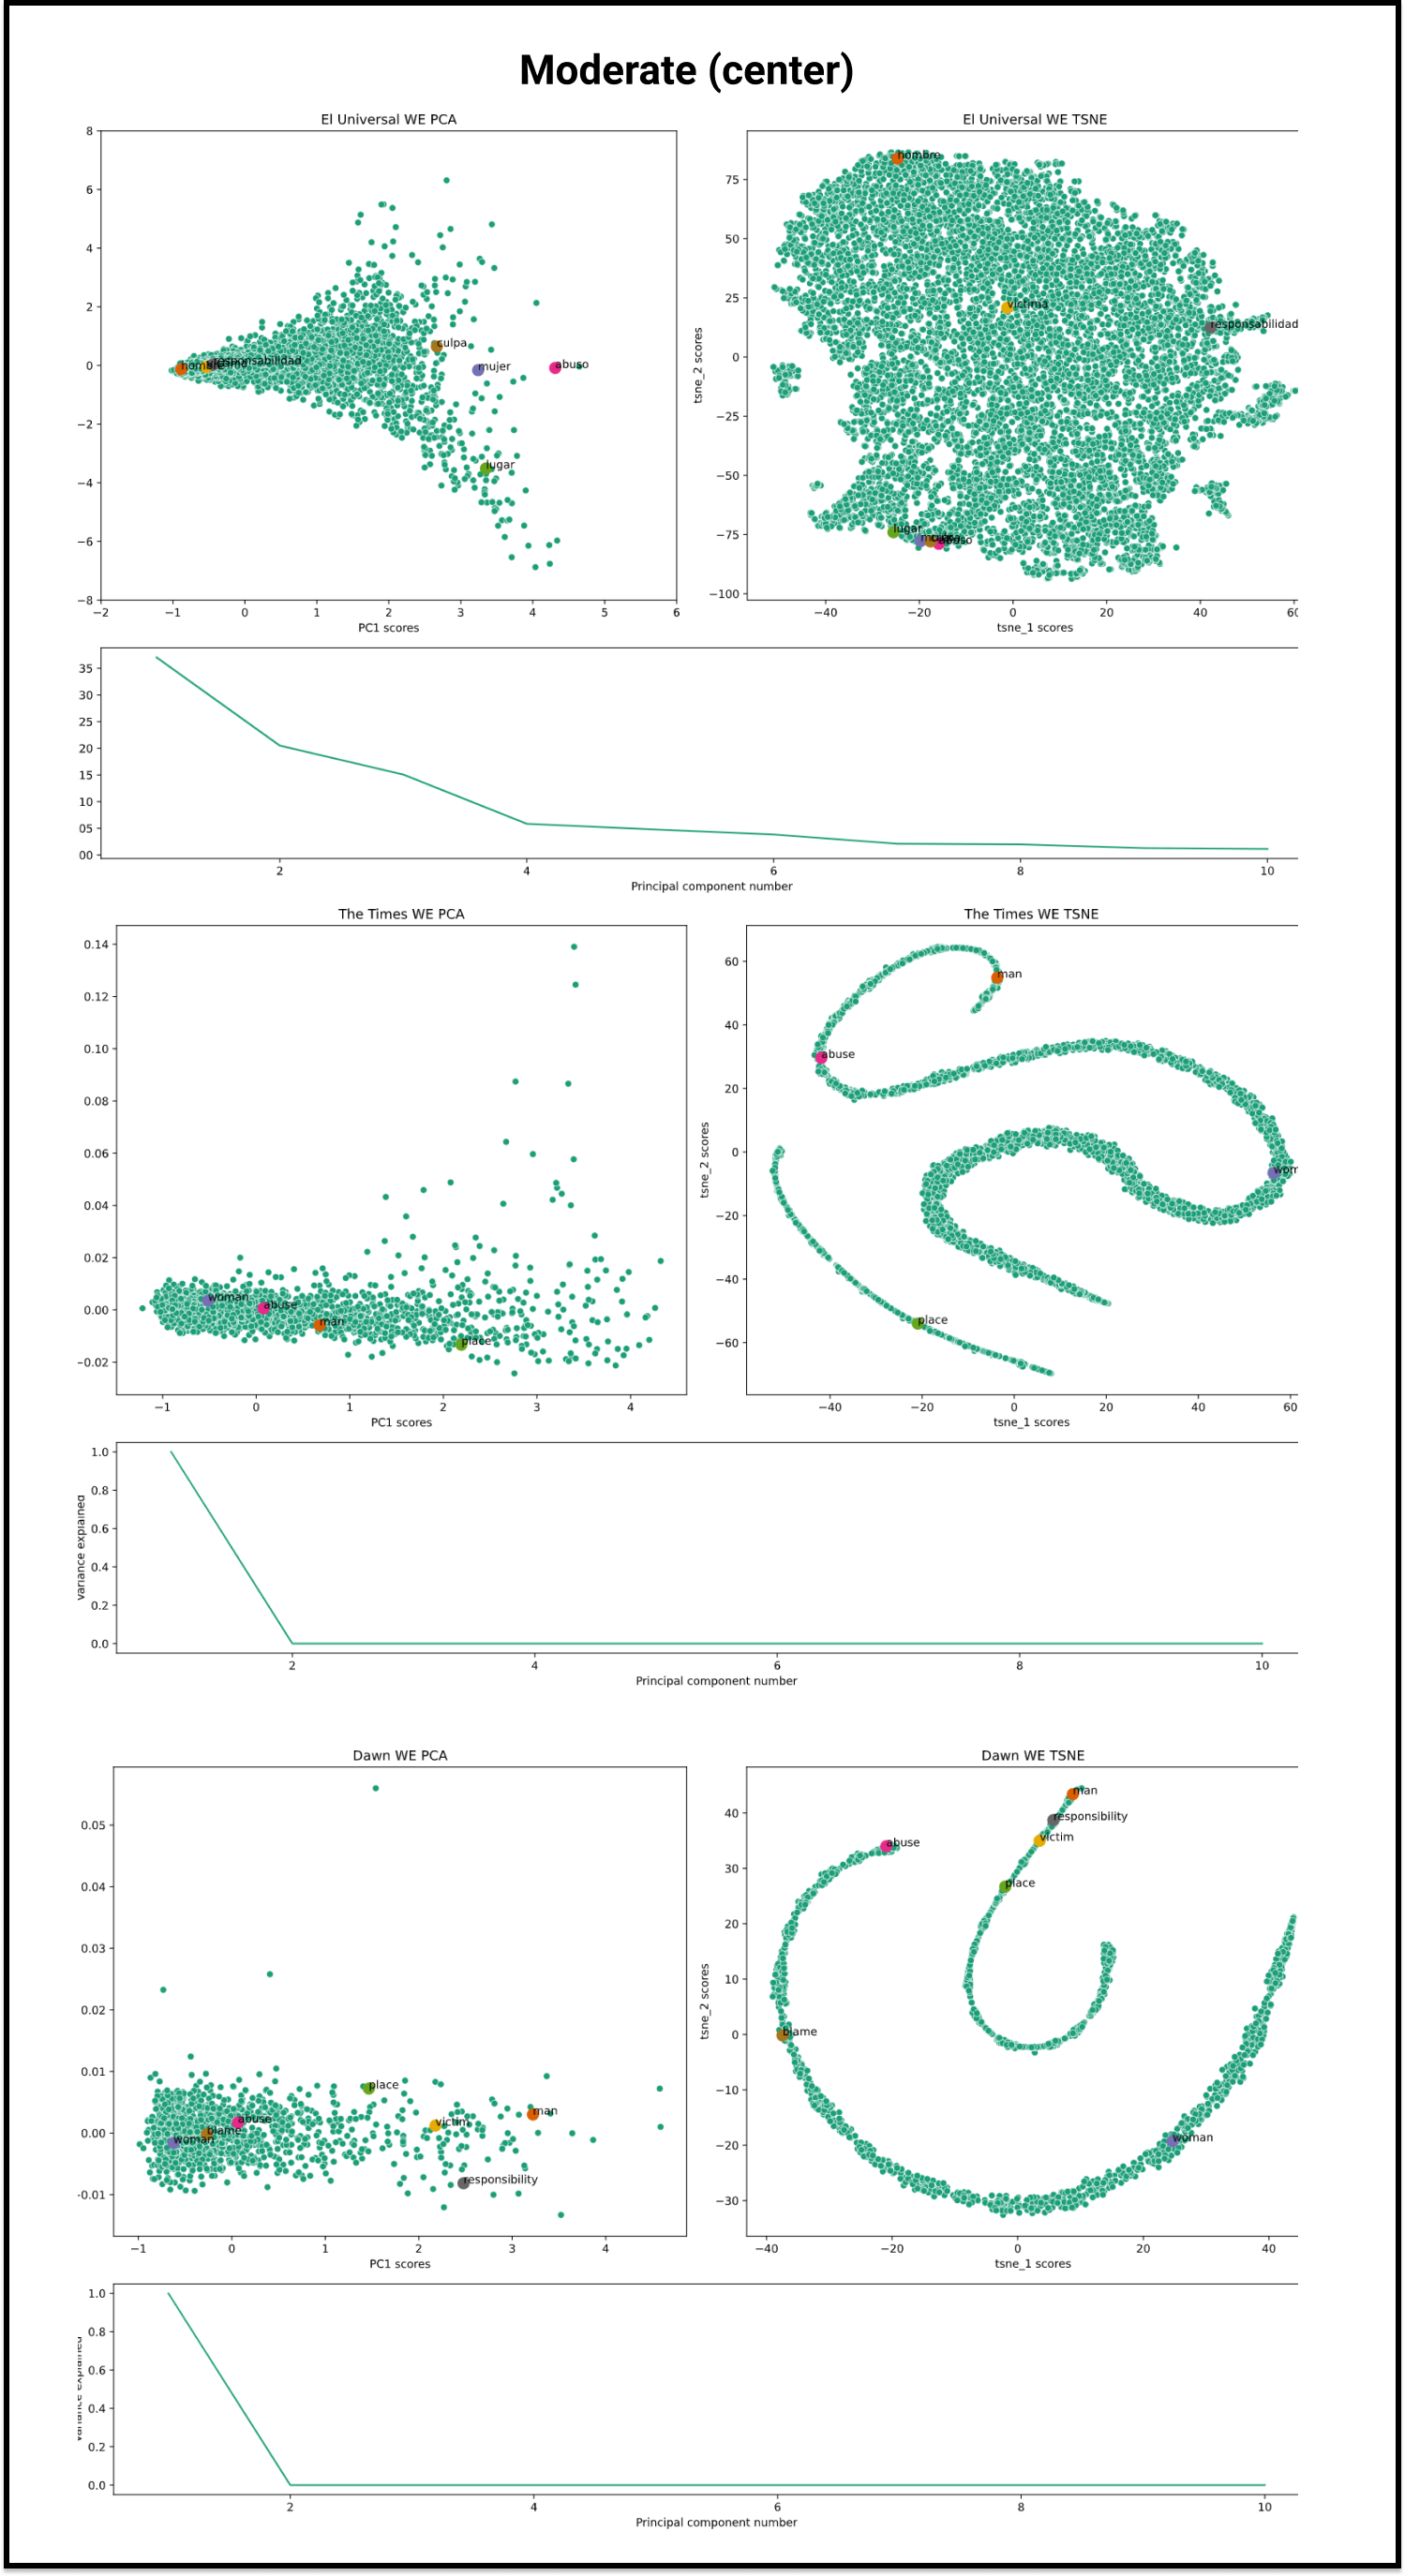
\includegraphics[width=\textwidth,height=\textheight,keepaspectratio]
		{figures/centerwe.png}}
	\caption{\label{fig:my-label1} GBV depiction in moderate media}
\end{figure}

\begin{figure}[H]
	\center{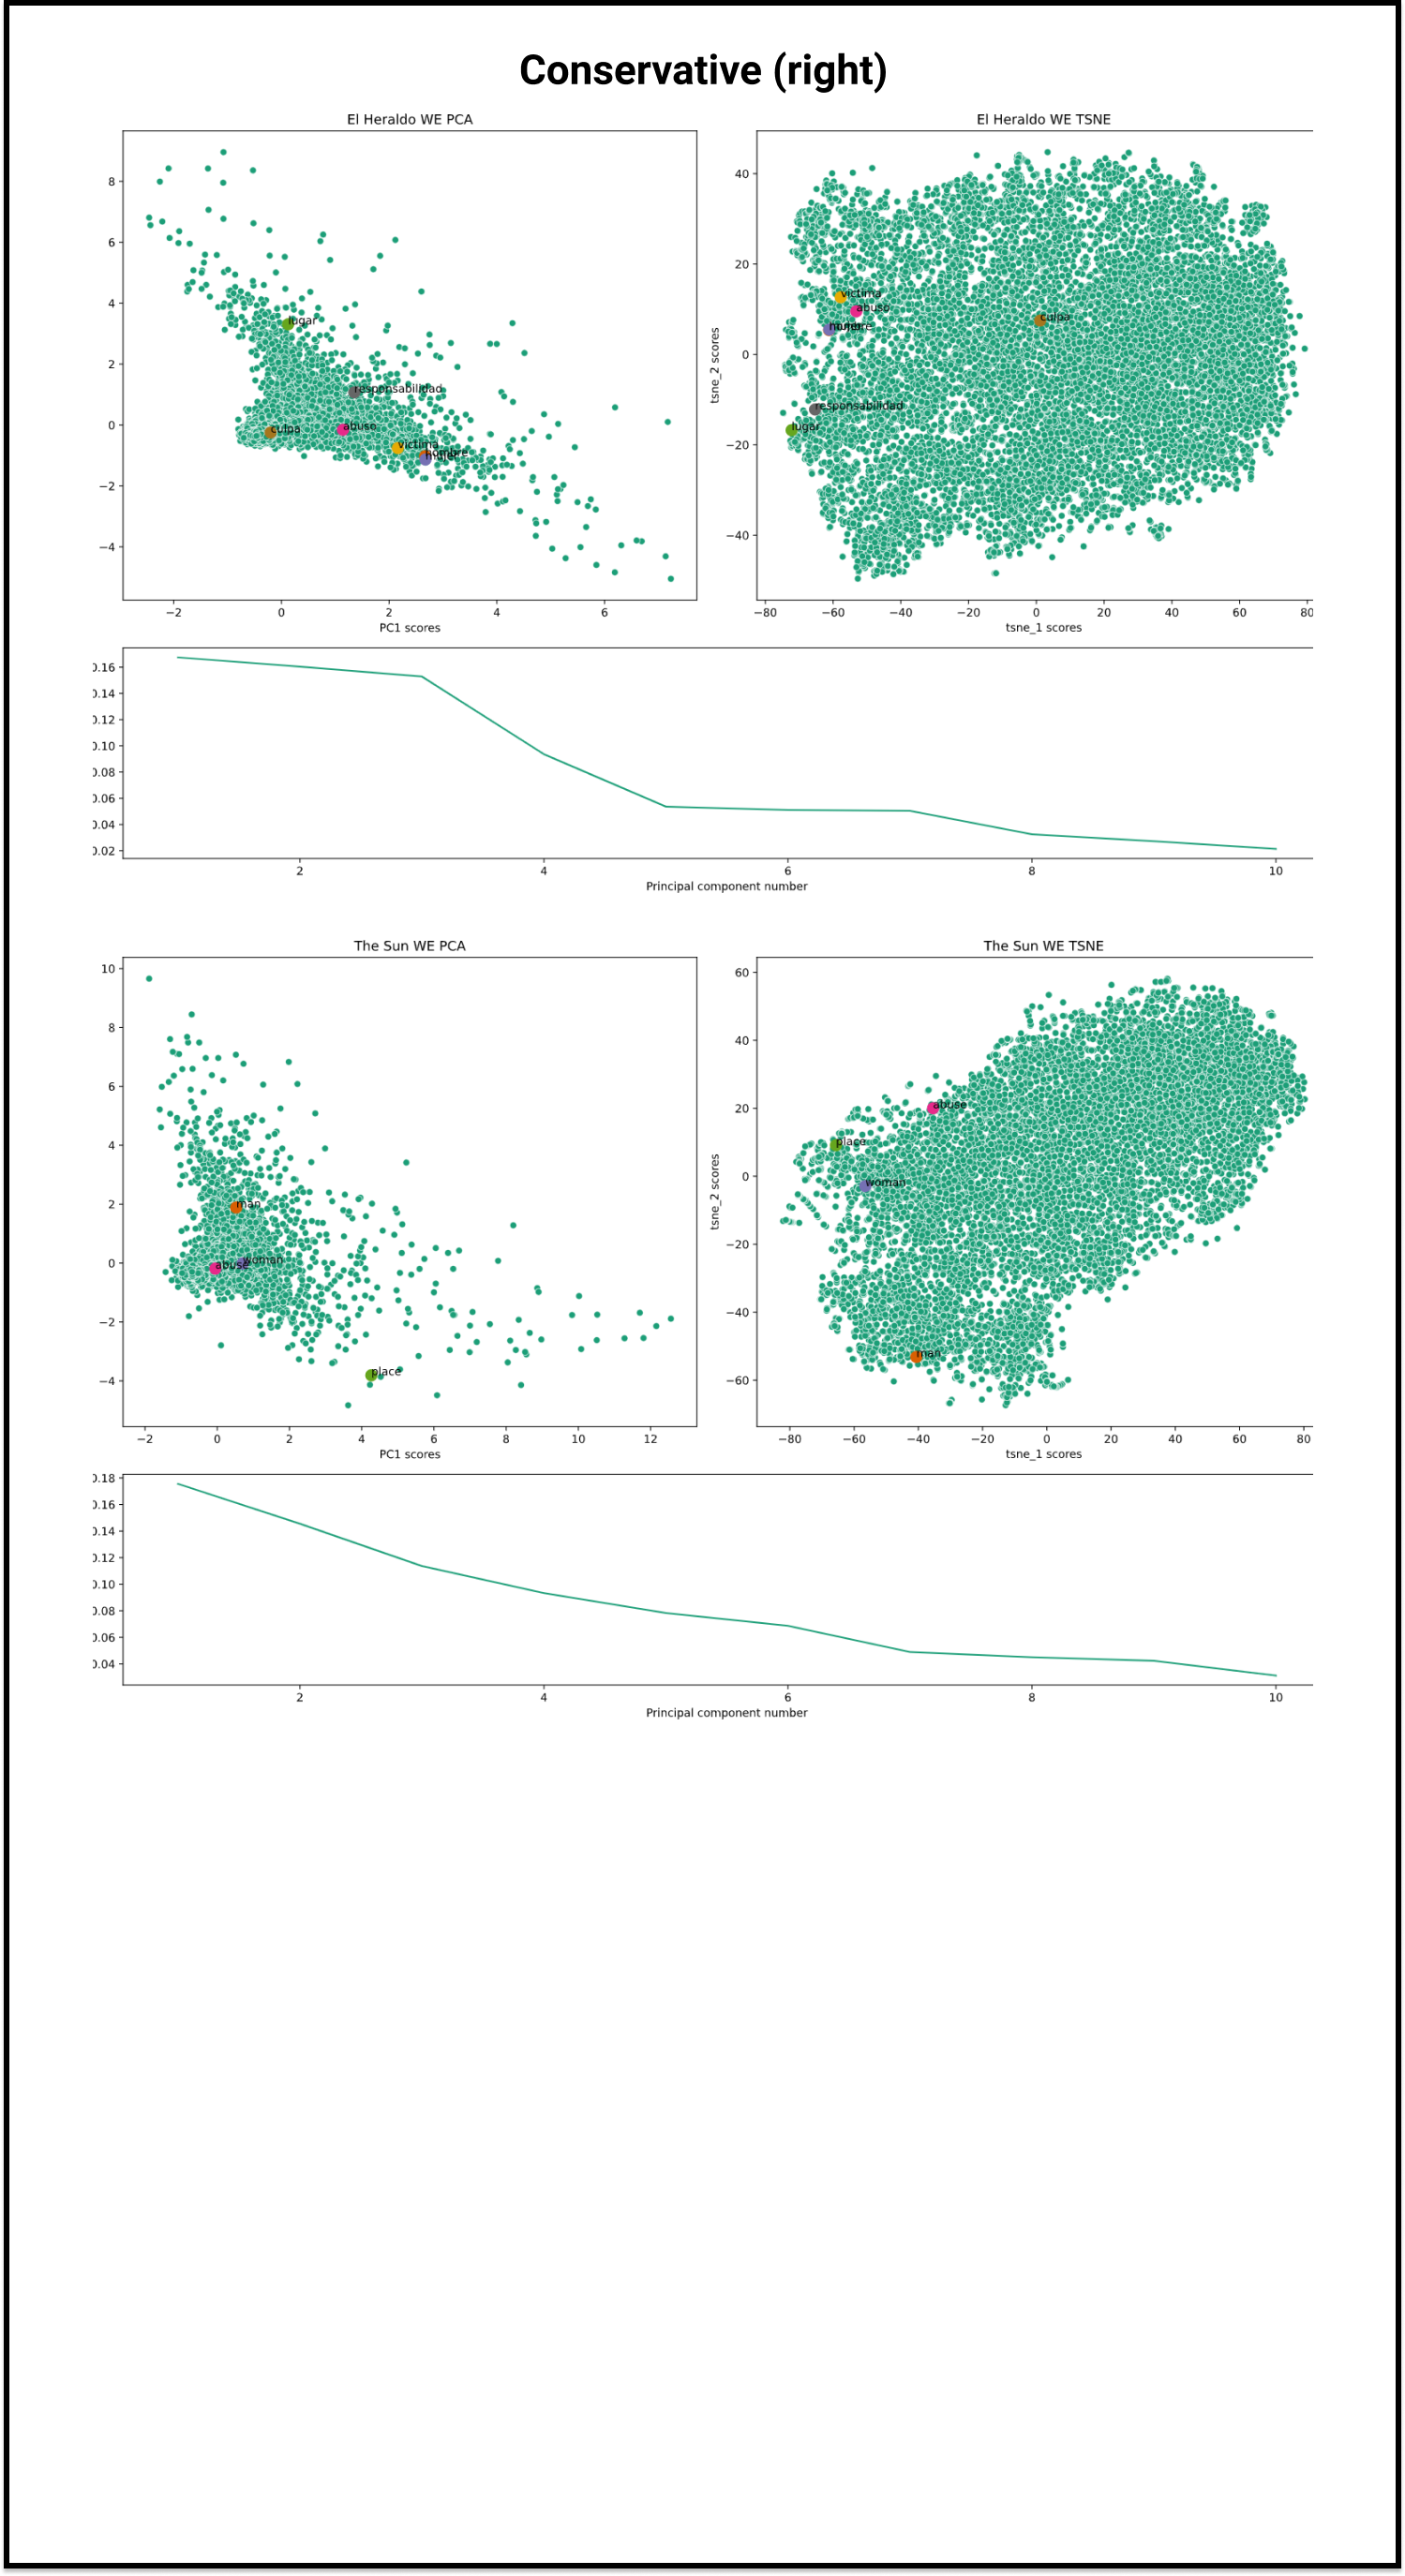
\includegraphics[width=\textwidth,height=\textheight,keepaspectratio]
		{figures/rightwe.png}}
	\caption{\label{fig:my-label1} GBV depiction right leaning media}
\end{figure}

}

\begin{figure}[H]
	\center{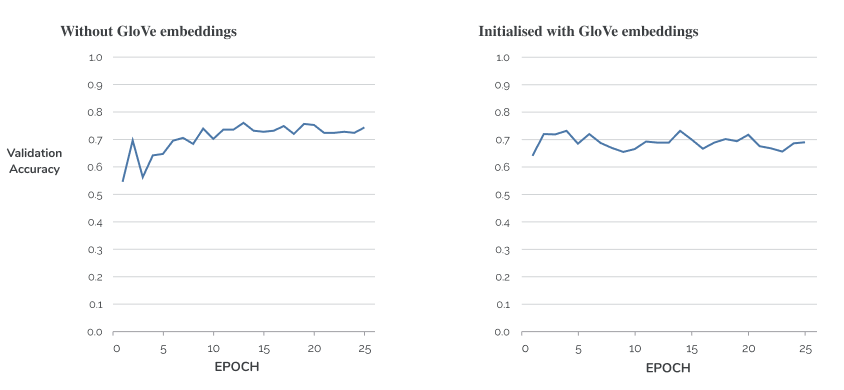
\includegraphics[width=\textwidth,height=\textheight,keepaspectratio]
		{figures/uk_validation_accuracies.png}}
	\caption{\label{fig:my-label1} UK LSTM models validation accuracy by EPOCH}
\end{figure}

\begin{figure}[H]
	\center{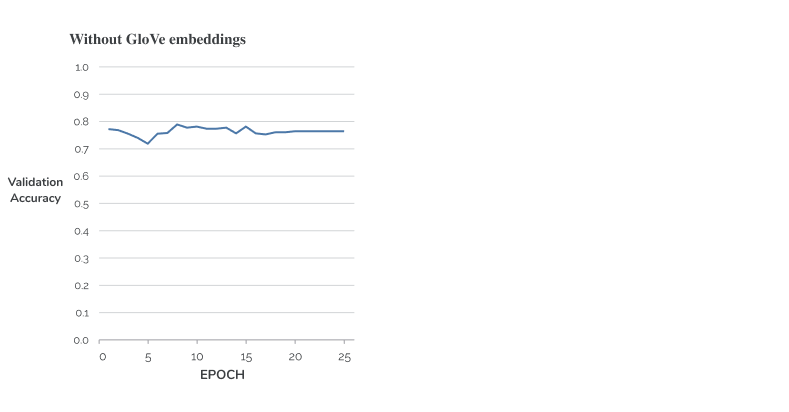
\includegraphics[width=\textwidth,height=\textheight,keepaspectratio]
		{figures/mexico_validation_accuracies.png}}
	\caption{\label{fig:my-label1} Mexico LSTM model validation accuracy by EPOCH}
\end{figure}



\section{References}\label{sec_ref}

[1] Bello, H. J., Palomar, N., Gallego, E., Navascués, L. J., and Lozano, C. (2020). Machine Learning to study the impact of gender-based violence in the news media. arXiv preprint arXiv:2012.07490.

[2] Busso, L., Combei, C. R., amd Tordini, O. (2020). Narrating Gender Violence A Corpus-Based Study on the Representation of Gender-Based Violence in Italian Media. In G. Giusti, and G. Iannàccaro (Eds.), Language, Gender and Hate Speech : A Multidisciplinary Approach (Language, Gender and Hate Speech A Multidisciplinary Approach). https://doi.org/10.30687/978-88-6969-478-3/002

[3] , A., Bryson, J. J., and Narayanan, A. (2017). Semantics derived automatically from language corpora contain human-like biases. Science, 356(6334), 183-186. doi:10.1126/science.aal4230

[4]Bail, C. A. (2012). The fringe effect. American Sociological Review, 77(6), 855-879. doi:10.1177/0003122412465743

[5]Kozlowski, A. C., Taddy, M., and Evans, J. A. (2019). The geometry of culture: Analyzing the meanings of class through word embeddings. American Sociological Review, 84(5), 905-949. doi:10.1177/0003122419877135

[6]Sendén, M. G., Sikström, S., and Lindholm, T. (2015). “She” and “He” in news media messages: Pronoun use reflects gender biases in semantic contexts. Sex Roles, 72(1-2), 40-49. doi: 10.1007/s11199-014-0437-x

[7]Von Nordheim, G., Muller, H., and Scheppe, M. (2019). Young, free and biased: A comparison of mainstream and right-wing media coverage of the 2015–16 refugee crisis in German newspapers. Journal of Alternative and Community Media, 4(1), 38-56. doi:10.1386/joacm000421
 
[8]Grimmer J. \& Stewart B.M (2013): Text as Data: The Promise and Pitfalls of Automatic Content Analysis Methods for Political Texts. 
{\it Political Analysis}

[9] V. Rodelo, Frida, and Carlos Muñiz. “La Orientación Política Del Periódico y Su Influencia En La Presencia De Encuadres y Asuntos Dentro De Las Noticias.” Estudios Sobre El Mensaje Periodístico, vol. 23, no. 1, 1970, pp. 241–256., doi:10.5209/esmp.55594. 

[10] Harris, Zellig S. “Distributional Structure.” Papers on Syntax, 1981, pp. 3–22., doi:10.1007/978-94-009-8467-71. 

[11] Tomas Mikolov, Ilya Sutskever, Kai Chen, Greg Corrado, and Jeffrey Dean. 2013. Distributed representations of words and phrases and their compositionality. In Proceedings of the 26th International Conference on Neural Information Processing Systems - Volume 2 (NIPS'13). Curran Associates Inc., Red Hook, NY, USA, 3111–3119.

[12] Gerd Bohner. 2001. Writing about rape: Use of the passive voice and other distancing text features as an expression of perceived responsibility of the victim. British Journal of Social Psychology. pp. 515–529 
\newpage
\pagebreak




\end{document}
